\subsection{Idealised model of an alt}
\label{sec:idealisedAlt}

%%%%%%%%%%

\begin{figure}% [thbp]
\begin{center}
\def\height{10mm} % height of boxes
\def\linW{15mm} % width of "Lin(t)" box
\def\gap{0.1} % gap for stacked figure
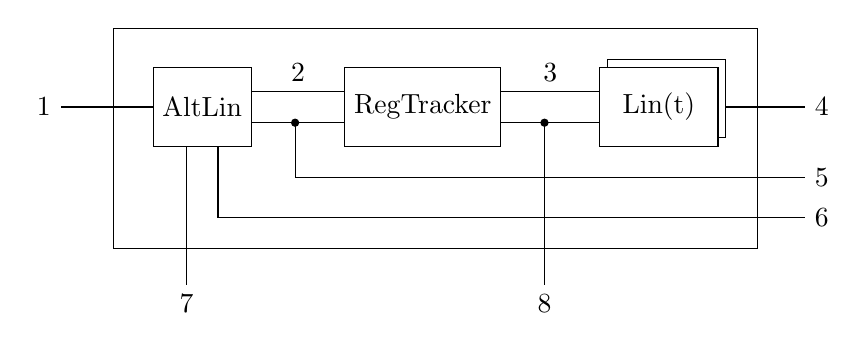
\begin{tikzpicture}
%%%%% AltLin
\draw(0,0) node[draw, minimum height = \height](altSpec){\cspmstyle AltLin};
%% (1)
\draw (altSpec) -- node[left, at end]{\inCircle{1}} ++ (-1.8, 0) 
  coordinate (left); 
%% (7)
\draw (altSpec.south) ++ (-0.2,0) -- node[below, at end]{\inCircle{7}}
   ++ (0,-1.75) coordinate (bottom);
%%%%% RegTracker
\draw (2.8,0) node[draw, minimum height = \height](regTracker){%
  \cspmstyle RegTracker};
%% Syncs between AltLin and RegTracker
\path (altSpec.east) -- ++(0,-0.2) coordinate (a) -- ++(0,0.4) coordinate (aa);
\path (regTracker.west) -- ++(0,-0.2) coordinate (b) -- 
  ++(0,0.4) coordinate (bb);
% (2)
\draw (aa) -- node[above]{\inCircle{2}} (bb);
%%%%% Lin
\draw (regTracker) ++ (3,0) 
  node[draw, minimum height = \height, minimum width = \linW](lin){
    \cspmstyle Lin(t)};
\draw (lin.north west) ++ (\gap, 0.0) |- ++ (\linW, \gap) |- 
  ++ (-\gap, -\height);
%% External coms
%% (4)
\draw (lin.east) ++ (0.1,0) -- node[right, at end]{\inCircle{4}} ++ (1.0,0)
coordinate (right);
%% (6)
\draw (altSpec.south) ++ (0.2,0) -- ++ (0,-0.9) coordinate (temp) -- 
  node[right, at end]{\inCircle{6}} (temp -| right); % (c);
%% (5)
\draw (a) -- (b);  
\fill  (a) ++ (0.55,0) circle(1.5pt) coordinate (t1);
\draw (t1) -- ++ (0,-0.7) coordinate (temp) --
  node[right, at end]{\inCircle{5}} (temp -| right); 
%% (9)
%% \draw (lin.south) -- node[below, at end]{\inCircle{9}}  (lin.south |-bottom);

%% Syncs between RegTracker and Lins
%% (3)
\path (regTracker.east) -- ++ (0,0.2) coordinate (l1) -- 
  ++(0,-0.4) coordinate (l2);
\path (lin.west) -- ++ (0,0.2) coordinate (r1) -- 
  ++(0,-0.4) coordinate (r2);
\draw (l1) -- node[above]{\inCircle{3}} (r1);
%% (8)
\draw (l2) -- (r2);
\fill (l2) ++ (0.55,0) circle(1.5pt) coordinate (temp);
\draw (temp) -- node[below, at end]{\inCircle{8}} (temp |- bottom);
%%%%% Outer box
\path (altSpec.west) -- ++ (-0.5,1) coordinate (a) -- ++(0,-2.8) coordinate (d);
\path (lin.east) --  ++(0.5,1) coordinate (b) -- ++(0,-2.8) coordinate (c);
\draw (a) -- (b) -- (c) -- (d) -- (a);
\end{tikzpicture}
\end{center}

%%%%%%%%%%%

\textbf{Key.} The interface with the alt-thread appears on the left; the
interface with channels appears on the right; error events and spurious
wakeups appear below; internal events appear inside the box.  

\raggedright
%
\begin{itemize}
\item[\inCircle{1}:] \CSPM{(begin}\m\CSPM{end)Alt};

\item[\inCircle{2}:] \CSPM{beginRegistration}, \CSPM{endRegistration},
  \CSPM{getToDeregister(In}\m\CSPM{Out)}, \CSPM{deregisterDone},
  \CSPM{endWait}; 

\item[\inCircle{3}:] \CSPM{maybe(Send}\m\CSPM{Receive)}, \CSPM{portClosed};

\item[\inCircle{4}:] \CSPM{(begin}\m\CSPM{end)Maybe(Send}\m\CSPM{Receive)},
  \CSPM{(begin}\m\CSPM{end)PortClosed}; 

\item[\inCircle{5}:] \CSPM{endRegister(In}\m\CSPM{Out)},
  \CSPM{endDeregister(In}\m\CSPM{Out)};   

\item[\inCircle{6}:] \CSPM{beginRegister(In}\m\CSPM{Out)},
  \CSPM{beginDeregister(In}\m\CSPM{Out)};   

\item[\inCircle{7}:] \CSPM{spuriousWakeup.AltThread}; 

\item[\inCircle{8}:] \CSPM{maybe(Send}\m\CSPM{Receive)Error}, 
  \CSPM{portClosedError}.

%% \item[\inCircle{9}:] \CSPM{spuriousWakeup.t}.
\end{itemize}
%
\caption{Construction of the idealised alt.  \label{fig:idealised-alt}}
\end{figure}

%%%%%%%%%%

We now give an idealised model of an alt.  As with the idealised channel, the
idealised alt identifies when its environment breaks the alt protocol, and
signals via an appropriate error event.  

We assume the definition of a value |branches| defining the branches of the
alt, as a sequence of values |InPortBranch.c| and |OutPortBranch.c| for
channels~|c|.  We assume a single alt-thread, |AltThread|, and a collection
|ChanThreads| of channel-threads.

The idealised alt is constructed from several components, as depicted in
Figure~\ref{fig:idealised-alt}.  The component |RegTracker| keeps track of
registrations of the alt at ports, or whether those ports are closed.  Each
component |Lin(t)| linearises callbacks by channel-thread~|t|.  The component
|AltLin| linearises the main call of the alt by the alt-thread.  We describe
these components in more detail below.

%%%%%%%%%%

\begin{figure}
\begin{cspm}
Lin(t) = 
  beginMaybeReceive.t?index?x -> LinMaybeReceive(t, index, x)
  [] beginMaybeSend.t?index -> LinMaybeSend(t, index)
  [] beginPortClosed.t?index -> LinPortClosed(t, index)
  
LinMaybeReceive(t, index, x) = 
  maybeReceive.t.index.x?res -> endMaybeReceive.t.res -> Lin(t)
  [] maybeReceiveError.t.index -> STOP
  
LinMaybeSend(t, index) = 
  maybeSend.t.index?res -> endMaybeSend.t.res -> Lin(t)
  [] maybeSendError.t.index -> STOP
  
LinPortClosed(t, index) = 
  portClosed.t.index -> endPortClosed.t -> Lin(t)
  [] portClosedError.t.index -> STOP
\end{cspm}
\caption{Definition of the {\scalastyle Lin(t)}
  processes.  \label{fig:alt-lin}} 
\end{figure}

%%%%%%%%%%

\paragraph{The {\scalashape Lin} processes.}

The |Lin(t)| processes, which linearise callbacks by channel-threads, are
defined in Figure~\ref{fig:alt-lin}.  Each accepts the |begin| event of a
callback function, which is handled by a different subsidiary process.  Each
callback may be either linearised correctly, or with an error event if it
breaks the alt protocol: the |RegTracker| process selects the appropriate
event, based on whether the alt is currently registered at the relevant port.

%%%%%%%%%%%%%%%%%%%%%%%%%%%%%%%%%%%%%%%%%%%%%%%%%%%%%%%%%%%%%%%%%

\paragraph{The {\scalashape AltLin} process.}

The |AltLin| process, which linearises the main calls of the alt, is defined
in Figure~\ref{fig:AltLin}. It initially signals to the |RegTracker| that it
is beginning registration, via event |beginRegistration|.  It then iterates
through |branches|, trying to register at each branch in turn, as described by
process |Register1| (the expression |nth(branches, i)| gives the branch at
index~|i|).  The |RegTracker| keeps track of the results of the registration
attempts.  If a registration is successful, |AltLin| moves to the
deregistration phase.

%%%%%%%%%%

\begin{figure}
\begin{cspm}
AltLin = beginAlt.AltThread -> beginRegistration -> Register(0)
  
Register(i) = 
  if i==size then endRegistration?ac -> (if ac then endAlt.AltThread.AltAbort -> AltLin else Waiting)
  else Register1(i, nth(branches,i))
  
Register1(i, InPortBranch.c) = 
  beginRegisterIn.AltThread.c.i -> (
    endRegisterIn.AltThread.c.RegisterSuccess?x -> Deregister(AltReceive.i.x)
    [] endRegisterIn.AltThread.c.RegisterWaiting -> Register(i+1)
    [] endRegisterIn.AltThread.c.RegisterClosed -> Register(i+1)
  )

Register1(i, OutPortBranch.c) =
  beginRegisterOut.AltThread.c.i -> (
    endRegisterOut.AltThread.c.RegisterSuccess?x -> Deregister(AltSend.i.x)
    [] endRegisterOut.AltThread.c.RegisterWaiting -> Register(i+1)
    [] endRegisterOut.AltThread.c.RegisterClosed -> Register(i+1)
  )
  
Deregister(result) =
  getToDeregisterIn?c.i -> beginDeregisterIn.AltThread.c.i ->
     endDeregisterIn.AltThread.c -> Deregister(result)
  [] getToDeregisterOut?c.i -> beginDeregisterOut.AltThread.c.i ->
        endDeregisterOut.AltThread.c -> Deregister(result)
  [] deregisterDone -> endAlt.AltThread.result -> AltLin
  
Waiting = 
  endWait?result -> (if result==AltAbort then endAlt.AltThread.result -> AltLin else Deregister(result))
  [] (spuriousWakeup.AltThread -> Waiting |~| STOP)
\end{cspm}
\caption{Definition of the {\scalastyle AltLin}
  processes.  \label{fig:AltLin}} 
\end{figure}

%%%%%%%%%%

If the registration phase gets to the end of |branches| without a successful
registration, it synchronises with |RegTracker| on channel |endRegistration|
to indicates to |RegTracker| that registration is over.  |AltLin| receives
from |RegTracker| a boolean, denoted~|ac|, that indicates whether all ports
have been closed; if so, the call on the alt returns with an |AltAbort|;
otherwise, the |AltLin| moves to the waiting phase.

The deregistration phase is defined by the process |Deregister(result)| (where
|result| will be the result of the call of the alt).  It repeatedly gets from
|RegTracker| information about a port to be deregistered, calls the relevant
deregistration function, and waits for it to return.  When there are no more
ports to deregister, |RegTracker| signals this on |deregisterDone|, at which
point |AltLin| ends the call on the alt. 

The waiting phase is defined by the process |Waiting|.  It waits for a
synchronisation on channel |endWait| with |RegTracker|, as a result of a
successful callback.  The |endWait| event contains the result of the call to
alt: if this is an |AltAbort|, |AltLin| simply returns; otherwise it moves to
the deregistration phase.  In addition, the process might have a spurious
wakeup while waiting, corresponding to event |spuriousWakeup.AltThread|. 

%%%%%%%%%%

\begin{figure}
\begin{cspm}
RegTracker = 
  beginRegistration -> RegTracker1(£%
    $\set{\CSPMMR{i} \mapsto \CSPMMR{NoReg} \mid 
       0 \le \CSPMMR{i} < \CSPMMR{length(branches})}$£) 
  [] maybeReceiveError?t?index -> STOP
  [] maybeSendError?t?index -> STOP
  [] portClosedError?t?index -> STOP
  
RegTracker1(reg) = 
  endRegisterIn.AltThread?c!RegisterWaiting -> 
    RegTracker1(reg£%
      $\null\oplus \set{\CSPMMR{indexFor(InPortBranch.c)} \mapsto 
         \CSPMMR{InPortReg.c}}$£)
  [] endRegisterOut.AltThread?c!RegisterWaiting -> 
       RegTracker1(reg£%
      $\null\oplus \set{\CSPMMR{indexFor(OutPortBranch.c)} \mapsto 
         \CSPMMR{OutPortReg.c}}$£)
  [] endRegisterIn.AltThread?c!RegisterClosed -> 
       RegTracker1(reg£%
      $\null\oplus \set{\CSPMMR{indexFor(InPortBranch.c)} \mapsto 
         \CSPMMR{Closed}}$£) 
  [] endRegisterOut.AltThread?c!RegisterClosed -> 
       RegTracker1(reg£%
      $\null\oplus \set{\CSPMMR{indexFor(OutPortBranch.c)} \mapsto 
         \CSPMMR{Closed}}$£)
  [] endRegisterIn.AltThread?c!RegisterSuccess?x -> RegTracker2(reg)
  [] endRegisterOut.AltThread?c!RegisterSuccess?x -> RegTracker2(reg)
  [] let ac = allClosed(reg) within endRegistration!ac -> (if ac then RegTracker else RegTracker3(reg))

RegTracker2(reg) = 
  let inRegs = getInRegs(reg) 
      outRegs = getOutRegs(reg)
      allRegs = inRegs £$\union$£ outRegs within
  (**[] (i£$\null \mapsto \CSPMMR{InPort.c}$£): reg @ getToDeregisterIn.c.i -> RegTracker2(reg) )
  [] (**[] (i£$\mapsto \CSPMMR{OutPortReg.c}$£): reg @ getToDeregisterOut.c.1 -> RegTracker2(reg) )
  [] allRegs=={} & deregisterDone -> RegTracker
  [] endDeregisterIn.AltThread?c -> RegTracker2(reg£%
      $\null\oplus \set{\CSPMMR{indexFor(InPortBranch.c)} \mapsto 
         \CSPMMR{NoReg}}$£)
  [] endDeregisterOut.AltThread?c -> RegTracker2(reg£%
      $\null\oplus \set{\CSPMMR{indexFor(OutPortBranch.c)} \mapsto 
         \CSPMMR{NoReg}}$£)
  [] maybeReceive?t?index:inRegs?x!false -> RegTracker2(reg£%
   $\null\oplus \set{\CSPMMR{index} \mapsto \CSPMMR{NoReg}}$£) 
  [] maybeSend?t?index:outRegs!None -> RegTracker2(reg£%
    $\null\oplus \set{\CSPMMR{index} \mapsto \CSPMMR{NoReg}}$£)
  [] portClosed?t?index:allRegs -> RegTracker2(reg£%
    $\null\oplus \set{\CSPMMR{index} \mapsto \CSPMMR{Closed}}$£)
  [] maybeReceiveError?t?index:Index-inRegs -> STOP
  [] maybeSendError?t?index:Index-outRegs -> STOP
  [] portClosedError?t?index:Index-allRegs -> STOP

RegTracker3(reg) = 
  let inRegs = getInRegs(reg) 
      outRegs = getOutRegs(reg)
      allRegs = inRegs £$\union$£ outRegs within
  maybeReceive?t?index:inRegs?x!true -> endWait.AltReceive.index.x -> 
     RegTracker2(reg£%
    $\null\oplus \set{\CSPMMR{index} \mapsto \CSPMMR{NoReg}}$£)
  [] (**|~| x : Data @ maybeSend?t?index:outRegs!Some.x -> endWait.AltSend.index.x -> 
        RegTracker2(reg£$\null\oplus \set{\CSPMMR{index} \mapsto \CSPMMR{NoReg}}$£))
  [] portClosed?t?index:allRegs -> 
        (let reg' = reg£%
      $\null\oplus \set{\CSPMMR{index} \mapsto \CSPMMR{Closed}}$£ within
         if allClosed(reg') then endWait.AltAbort -> RegTracker else RegTracker3(reg'))
  [] maybeReceiveError?t?index:Index-inRegs -> STOP
  [] maybeSendError?t?index:Index-outRegs -> STOP
  [] portClosedError?t?index:Index-allRegs -> STOP
\end{cspm}
\caption{The {\scalastyle RegTracker} process. 
%, {\scalastyle RegTracker1} and {\scalastyle RegTracker2} processes.
\label{fig:RegTracker}}
\end{figure}

%RecordDereg(reg, OutPortReg.c)
%RecordDereg(reg, InPortReg.c)
%RecordClosed(reg, OutPortBranch.c)
% RecordClosed(reg, InPortBranch.c)
%     RecordReg(reg, OutPortBranch.c, OutPortReg.c)
%    RecordReg(reg, InPortBranch.c, InPortReg.c)
%% RecordReg(reg, branch, portReg) = extractSingle(
%%   branchesFor(branch), 
%%   £$\lambda$£index @ expect(reg(index)==NoReg, RegTracker1(reg£%
%%     $\null\oplus \set{\CSPMMR{index} \mapsto \CSPMMR{portReg}}$£) )
%% ) 

%% RecordClosed(reg, portReg) = extractSingle(
%%   branchesFor(portReg),
%%   £$\lambda$£index @ expect(reg(index)==NoReg, RegTracker1(reg£%
%%     $\null\oplus \set{\CSPMMR{index} \mapsto \CSPMMR{Closed}}$£) )  
%% )

%%%%%%%%%%

\paragraph{The {\scalashape RegTracker} process.}

The |RegTracker| process is defined starting in Figure~\ref{fig:RegTracker}.
It waits to receive notification, via event |beginRegistration| that
registration has started.  However, any callback before this point would be
outside the alt protocol, in which case it signals an error.

Each subsidiary process has a parameter |reg|, which is a mapping from
indices of |branches| to the type |RegInfo|, defined as follows.
%
\begin{cspm}
  datatype RegInfo = NoReg | InPortReg.ChanID | OutPortReg.ChanID | Closed
\end{cspm}
%
The clauses in |RegInfo| represent, respectively, that the corresponding
branch is not registered, registered at an inport, registered at an outport,
or the port is closed.  Initially all indices are marked as not registered.

The process |RegTracker1| synchronises on the |end| events of call to
|registerIn| and |registerOut|.  In the case of a |RegisterWaiting| or
|RegisterClosed| result, |reg| is updated to map the relevant index to an
appropriate value.
%
If a registration attempt is successful, the process moves to state
|RegTracker2|, corresponding to the deregistration phase, described below.  If
the |AltLin| synchronises on |endRegistration|, indicating the end of the
registration phase, the |RegTracker| sends a value indicating whether all the
ports have been closed (calculated using the helper function |allClosed|); if
so, it returns to its initial state; otherwise it moves to state
|RegTracker3|, corresponding to the waiting phase.
%
Note that during the registration phase, |RegTracker| blocks all callbacks,
reflecting the behaviour of the implementation. 

%% the subsidiary process \CSPM{RecordReg} (omitted for brevity) updates |reg| so
%% the relevant index maps to the |portReg|.
%% calls \CSPM{RegTracker1(reg}$\null\oplus \set{\CSPMMR{index} \mapsto
%% \CSPMMR{portReg}}$\CSPM{)}.
%% Likewise, \CSPM{RecordClosed(reg, branch)} updates |reg| so the index maps to
%% |Closed|.

%% calls \CSPM{RegTracker1(reg}$\null\oplus \set{\CSPMMR{index} \mapsto
%%   \CSPMMR{Closed}}$\CSPM{)}.

%%%%%%%%%%

%% \begin{figure}
%% \begin{cspm}
%% RegTracker2(reg) = 
%%   let inRegs = getInRegs(reg) 
%%       outRegs = getOutRegs(reg)
%%       allRegs = inRegs £$\union$£ outRegs within
%%   (**[] (i£$\null \mapsto \CSPMMR{InPort.c}$£): reg @ getToDeregisterIn.c.i -> RegTracker2(reg) )
%%   []
%%   (**[] (i£$\mapsto \CSPMMR{OutPortReg.c}$£): reg @ getToDeregisterOut.c.1 -> RegTracker2(reg) )
%%   []
%%   allRegs=={} & deregisterDone -> RegTracker
%%   []
%%   endDeregisterIn.AltThread?c -> RecordDereg(reg, InPortReg.c)
%%   [] 
%%   endDeregisterOut.AltThread?c -> RecordDereg(reg, OutPortReg.c)
%%   []
%%   portClosed?t?index:allRegs -> RegTracker2(reg£%
%%     $\null\oplus \set{\CSPMMR{index} \mapsto \CSPMMR{Closed}}$£)
%%   []
%%   portClosedError?t?index:Index-allRegs -> STOP
%%   []
%%   maybeReceive?t?index:inRegs?_!false -> RegTracker2(reg£%
%%    $\null\oplus \set{\CSPMMR{index} \mapsto \CSPMMR{NoReg}}$£) 
%%   []
%%   maybeSend?t?index:outRegs!None -> RegTracker2(reg£%
%%     $\null\oplus \set{\CSPMMR{index} \mapsto \CSPMMR{NoReg}}$£)
%%   []
%%   maybeReceiveError?t?index:Index-inRegs -> STOP
%%   []
%%   maybeSendError?t?index:Index-outRegs -> STOP
%% \end{cspm}
%% \caption{The {\scalastyle RegTracker2} process.  \label{fig:RegTracker2}}
%% \end{figure}

%% RecordDereg(reg, portReg) = 
%%   let matches = matchesFor(reg, portReg) within 
%%   if matches == {} then RegTracker2(reg)
%%   else extractSingle(matches, £$\lambda$£index @ RegTracker2(reg£%
%%     $\null\oplus \set{\CSPMMR{index} \mapsto \CSPMMR{NoReg}}$£))

%%%%%%%%%%

The process |RegTracker2(reg)| deals with deregistration.  The names |inRegs|,
|outRegs| and |allRegs| are set to the indices of registered inports,
registered outports, and all registered ports, respectively.  The process can
send to |AltLin| information about a port that can be deregistered (channels
|getToDeregisterIn| and |getToDeregisterOut|), or an indication that there is
no such port (channel |deregisterDone|).  It synchronises on the |end| events
of deregistrations, and updates its state to map the relevant index to
|NoReg|.
%% (via the subsidiary process |RecordDereg|, omitted for brevity).

|RegTracker2| can synchronise with |Lin(t)| on the linearisation point of a
\SCALA{maybeReceive} operation corresponding to a registered inport; at this
point, the callback will be unsuccessful, as captured by the final |false|
field in the event.  Likewise, it can synchronise on the linearisation point
of a \SCALA{maybeSend} operation corresponding to a registered outport, which
again will be unsuccessful.  Further, it can synchronise on the linearisation
point of a \SCALA{closed} operation on a registered port.  However, any
callback not corresponding to a suitably registered port would be outside of
the alt protocol, so an error is signalled. 

%%%%%%%%%%

%% \begin{figure}
%% \begin{cspm}
%% RegTracker3(reg) = 
%%   let inRegs = getInRegs(reg) 
%%       outRegs = getOutRegs(reg)
%%       allRegs = inRegs £$\union$£ outRegs within
%%   maybeReceive?t?index:inRegs?x!true -> endWait.AltReceive.index.x -> RegTracker2(reg£%
%%     $\null\oplus \set{\CSPMMR{index} \mapsto \CSPMMR{NoReg}}$£)
%%   [] (**|~| x : Data @ maybeSend?t?index:outRegs!Some.x -> endWait.AltSend.index.x -> RegTracker2(reg£%
%%     $\null\oplus \set{\CSPMMR{index} \mapsto \CSPMMR{NoReg}}$£))
%%   [] portClosed?t?index:allRegs -> 
%%        (let reg' = reg£%
%%       $\null\oplus \set{\CSPMMR{index} \mapsto \CSPMMR{Closed}}$£ within if allClosed(reg') then endWait.AltAbort -> RegTracker else RegTracker3(reg'))
%%   [] maybeReceiveError?t?index:Index-inRegs -> STOP
%%   [] maybeSendError?t?index:Index-outRegs -> STOP
%%   [] portClosedError?t?index:Index-allRegs -> STOP
%% \end{cspm}
%% \caption{The {\scalastyle RegTracker3} process.  \label{fig:RegTracker3}}
%% \end{figure}

%%%%%%%%%%

The |RegTracker3| process %(Figure~\ref{fig:RegTracker3}) 
deals with the
waiting phase, waiting for callbacks from registered ports.  It can
synchronise with |Lin(t)| on the linearisation point of a \SCALA{maybeReceive}
operation corresponding to a registered inport.  The operation will be
successful, as captured by the final |true| field in the event.  It informs
|AltLin| of the success, on channel |endWait|, and moves to the deregistration
phase.  Likewise, it can synchronise on the linearisation point of a
\SCALA{maybeSend} operation corresponding to a registered outport; this
succeeds with a value~|x| sent (modelled as being chosen
nondeterministically).  Further, it can synchronise on the linearisation point
of a |close| operation; if all ports are now closed, it indicates this to
|AltSpec| on channel |endWait|.  However, any callback not corresponding to a
suitably registered port would be outside of the alt protocol, so an error is
signalled.

%%%%%%%%%%%%%%%%%%%%%%%%%%%%%%%%%%%%%%%%%%%%%%%%%%%%%%

%\begin{mysamepage}
\paragraph{Testing the idealised alt.}

The components are combined together, as illustrated in
Figure~\ref{fig:idealised-alt}, to produce a process |IdealisedAlt|.  We
then allow arbitrary behaviours after the error events, much as for the
idealised model of a channel.
%
\begin{cspm}
Errors£$_A$£ = {|maybeReceiveError, maybeSendError, portClosedError|}
AltSpec£$_F$£ = (IdealisedAlt [|Errors£$_A$£|> CHAOS(Interface) ) \ Errors£$_A$£
AltSpec£$_D$£ = (IdealisedAlt [|Errors£$_A$£|> DIV ) \ Errors£$_A$£
\end{cspm}
%\end{mysamepage}

We can then compare the CSP model of an alt implementation to the idealised
model.  We can verify that the implementation model refines |AltSpec|$_F$ and
|AltSpec|$_D$ in the relevant semantic models.

\begin{window}[1,r,{
%
\vspace{0.5ex}
\begin{tabular}{\|cccc\|}
Model & Threads & States  & Time\\
F & 4 & 33.1M & 21s \\
FD & 4 & 5.6M & 5.4s \\
F & 5 & 601M & 472s \\
FD & 5 & 62.7M & 46s \\
F & 6 & 10.6B & 153min \\
FD & 6 & 662M & 701s \\
%% F & 4 & 33.3M & 25s \\
%% FD & 4 & 5.7M & 6s  \\
%% F & 5 & 604M & 476s \\
%% FD & 5 & 63.8M & 47s  \\ % prev 39s ? 
%% F & 6 & 10.7B & 155min \\
%% FD & 6 & 672M & 713s
\end{tabular}
},]
%
The table to the right gives statistics about these checks.  In each case, we
considered an alt with two branches, one inport branch and one outport
branch.  The checks are faster than the corresponding checks for a channel,
mainly because normalisation of the specification was
faster than for a channel, because the idealised alt has fewer states than an
idealised channel.  We think the main reason for this is that the |Lin(t)|
processes in the idealised alt have fewer states than the |Lin(t)| processes
in the idealised channel (there is one such process for each channel thread,
so the total number of states increases exponentially).  In addition, the
implementation model for an alt has fewer states than for a channel.
\end{window}

We used a couple of techniques to improve the efficiency of these checks.
Firstly, we applied the prioritisation operator of FDR to |IdealisedAlt| to
give priority to error events over all other events (except $\tau$s); so in
any state where an error event (or $\tau$) is possible, all other events are
blocked.  This is sound here because the subsequent behaviours allowed by the
specification (in |CHAOS(Interface)| or |DIV|) include the behaviours
corresponding to the blocked events.

Further, for the check in the stable-failures model, we normalised
|IdealisedAlt| before the application of the throws operator.  This made the
subsequent normalisation of |AltSpec|$_F$ faster.  (However, the same
technique in the failures-divergences model made the check slower.)

% In idealised chan model also? -- doesn't seem to help
